\section{Techniques for planar graphs}\label{techniques}
In this section, we describe techniques popularly used in algorithms for planar graphs.
These techniques are also used to optimize our distance oracles in preprocessing time, space and
query times.

\subsection{Separators in planar graphs}\label{rdiv2}
A \textit{Jordan curve} is a simple closed curve in the plane. Given a planar graph $G$,
a Jordan curve separator is a curve that intersects $G$ only at vertices. In 1984, Miller
\cite{miller1984finding} showed that for any planar graph with $n$ vertices, there is a Jordan curve
separator of size $O(\sqrt{n})$ such that each new component contains at most $2n/3$
vertices. He further showed that such a separator can be found in $O(n)$ time. \\
Frederickson \cite{frederickson1987fast} introduced the \textit{$r$-division} for planar
graphs. Given an $r\in (0,n)$, the division is a decomposition of the graph into
$O(n/r)$ edge-induced subgraphs (\textit{pieces}), where each piece contains $O(r)$ vertices and $O(\sqrt{r})$ \textit{boundary vertices}. A
boundary vertex is a vertex that belongs to multiple pieces, while an \textit{interior
vertex} is one that belongs to a single piece. Frederickson showed that
such a division exists for any planar graphs and can be found in $O(n\lg n)$ time. This
was achieved by applying the separator theorem of Lipton and Tarjan
\cite{lipton1979separator}, which states that for any planar graphs, there is a separator
of size $O(\sqrt{n})$ that splits $G$ into two graph each containing at most $2n/3$ of
the vertices. Klein and Subramanain \cite{klein1998fully} were the first to give an
$r$-division which had \textit{few holes}. Holes are faces of a piece which are not faces
of the graph $G$. These occur when we separate the graph recursively. This was further developed
by Klein et al. \cite{klein2013structured}, who gave a $O(n)$ time algorithm to compute
an $r$-division of a planar graph $G$ also with the additional property that each piece has a
constant number of holes. It also produces a decomposition tree representing a recursive
decomposition of $G$. Particularly, given an increasing sequence $\overline{r}=(r_1,r_2,\dots)$, we
continue to decompose a piece on the previous level of the decomposition.
\\
The $r$-division we will use in this thesis (unless described otherwise) is the one by Klein et al.
\cite{klein2013structured} with a constant number of
holes with connected pieces, that provides a decomposition tree and can be computed in
linear time. That $r$-division guarantees the following:
\begin{lemma}\label{rdivlemma}
  The constructed $r$-division ensures that (i) each piece has $O(1)$ holes, (ii) the
  number of vertices in a piece on the $k$-th level in the decomposition is
  $O(n/c_1^{k/3})$ for some constant $c_1>1$, (iii) the number of boundary nodes in a
  piece on the $k$-th level in the decomposition is $O(\sqrt{n}/c_2^{k/3})$ for some
  constant $c_2>1$.
\end{lemma}
\noindent A proof of the Lemma can be found in \cite{klein2013structured}. \\
Summing over all levels of the decomposition gives us that the total number of boundary
vertices is $O(\sqrt{n})$.\\
An illustration of the components in an $r$-division is shown in Figure \ref{rdiv}. We give
a result based on an $r$-division in Section \ref{oracle1}.

\begin{figure}[h!]
  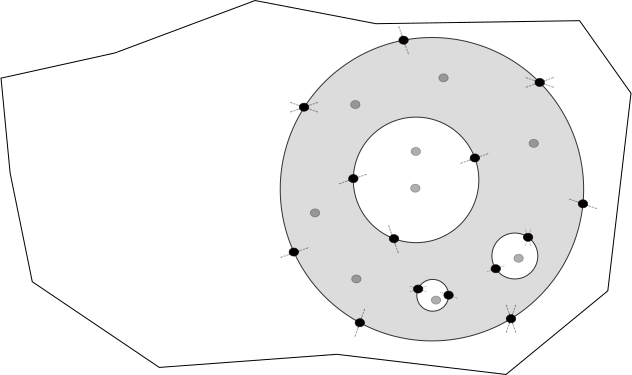
\includegraphics[width=1.0\textwidth]{figs/rdiv.pdf}
  \caption{Illustration of an $r$-division. A piece $P$ of the graph $G$ is shown in
  grey with holes in white. Boundary vertices are shown as black circles, interior vertices are shown in
grey. Any edge passing through the Jordan curve goes through a boundary vertex as
indicated by the arrows.}
    \label{rdiv}
\end{figure}

\subsection{Klein's multiple source shortest path}\label{klein2}
Klein's multiple source shortest path \cite{klein2005multiple} is another useful tool for planar
graphs. Given a planar graph with nonnegative weight, we can in $O(n\lg n)$ time construct a data structure
of size $O(n \lg n)$ that can answer queries of the following form in $O(\lg n)$ time:
For a source vertex $v$ and a vertex $b$ on the boundary of the infinite face, find the
shortest path from $v$ to $s$. This is especially useful to compute all pairs shortest paths between boundary
vertices in an $r$-division as it requires $O(r\lg r)$ time for a piece $P$ with
$|P|=O(r)$. \\
The idea is to compute a shortest path tree $T$ rooted at a boundary vertex
$b_i$ and then modifying the tree to get the shortest path tree rooted at the
neighbouring boundary vertex $b_{i+1}$. Using an efficient representation of dynamic
trees that allow operations to be done in amortized $O(\lg n)$ time is possible
\cite{tarjan2005self}\cite{henzinger1999randomized}. Any edge will then join the tree at
most once and leave the tree at most once. Since the graph is planar, we have $O(r)$ edges,
giving us the $O(r\lg r)$ running time. \\
The query idea is to use an Euler tour representation of the tree, called $T$, so we can
return the distance from a vertex $u$ to the root $r$ of the tree. Since we need the
correct version of the tree computed during preprocessing, we need a persistent data
structure that remembers changes to $T$, so we can recover any state of $T$. \\
An illustration to provide an intuition of the data structure is given in Figure
\ref{klein}.

\begin{figure}[h!]
  \centering
  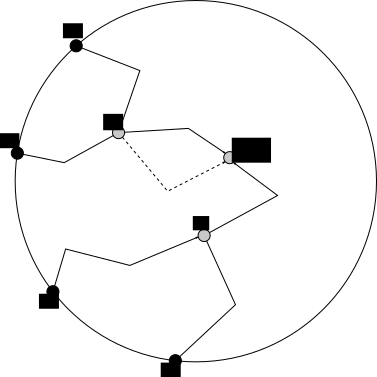
\includegraphics[width=0.6\textwidth]{figs/klein.pdf}
  \caption{Illustration of Klein's MSSP structure. The idea is two adjacent boundary
    vertices have almost identical shortest path trees. Computing shortest path trees
    $T_i$ clockwise
    around the face from $b_1$, we need only consider the \textit{differences} between
  the two trees. The dashed line is an impossible situation. Having computed the shortest
path tree rooted in $b_3$, $T_3$, where the shortest path to $v$ goes through $w$, it is
impossible for the shortest path tree rooted in $b_4$ to "cross" $T_3$ since it would
imply a shorter path from $w$ to $v$.}
    \label{klein}
\end{figure}

\subsection{The dense distance graph}
A \textit{dense distance graph} or DDG is defined over a decomposition of a planar
graph. Throughout this thesis, the decomposition is the $r$-division of $G$. It is the non-planar graph $G'$ of $G$ where there is an edge $uv$ if both $u$ and
$v$ are boundary vertices with weight equal to the shortest path between the vertices within
the piece(s) they share. The space requirement for storing the matrix of all distances between boundary
vertices in each piece is $O(\sqrt{r}^2)=O(r)$. We can construct it using Klein's multiple source shortest
path algorithm in $O(r\lg r)$ time since each piece has $O(1)$ holes.
Summing over all $O(n/r)$ pieces, the total space required is $O(n)$. Likewise, calculating all
distances in all pieces requires $O(nr\lg r/r)=O(n\lg r)$ time.

\subsection{Monge property}
Given two ordered sets $A$ and $B$ and a distance function $d$, we say $d$ has the
\textit{Monge property} if for elements $u, v\in A$ and $x, y\in B$, where
$u\leq v$ and $x\leq y$, then:
\begin{align*}
  d(u,x)+d(v,y)\leq d(u, y)+d(v,x)
\end{align*}
An example of this is shortest paths distances between boundary vertices in planar graph
given all four boundary vertices lie on the infinite face. It states that the sum of
paths that do not cross is at most the sum of paths that do cross. Figure \ref{monge}
illustrates this. \\
Another implication of the property is that if we have found the $u$ that minimizes $d(u,y)$,
then for all boundary vertices $v$ that are on  counter clockwise path on the face $f$
(according to Figure \ref{monge}), then $d(v,x)\geq d(u,x)$. To see this, note that there
is a vertex $w$ on path from $u$ to $y$ that the path $v$ to $x$ must cross. Since
$d(u,y)\leq d(v,y)$, it implies that $d(u,w)\leq d(v,w)$. It is important that all
vertices are on the boundary of the face as it is otherwise not true (as indicated by
Figure \ref{monge2}). \\
The \textit{Monge matching problem} is finding the parent $p(v)\in A$ for all $v\in B$,
so that $d(p(v), v)\leq d(u,v)$ for any $u\in A$. The \textit{minimum Monge matching} is
the set of $(p(v), v)$. This problem has a famous $O(m+n)$ solution for a $m$ by $n$ matrix found by Aggarwal et al.
\cite{aggarwal1987geometric}, and is also known as the SMAWK algorithm. The Monge property is used in the algorithm described in Section
\ref{frdjikstra} to speed up shortest path searching with Djikstra's algorithm using
\textit{Monge heaps}.

\begin{figure}
  \centering
  \begin{subfigure}[b]{0.45\textwidth}
    \includegraphics[width=\textwidth]{figs/monge.pdf}
    \caption{Illustration of the Monge property in planar graphs. The sum of the distances
  when paths cross (in solid) are less than or equal to the sum of distances when paths
do not cross (in dashed lines).}
    \label{monge}
  \end{subfigure}
  \quad
  \begin{subfigure}[b]{0.45\textwidth}
    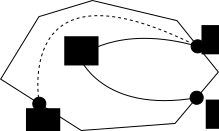
\includegraphics[width=\textwidth]{figs/monge2.pdf}
    \caption{A scenario where the Monge property does not hold, since paths
      do not cross. The shortest paths from $u$ are
      indicated by solid lines and a shorter path to $x$ is indicated by a dashed line.}
    \label{monge2}
  \end{subfigure}
\end{figure}

\subsubsection{The Monge subheap structure}\label{mongeheap}
FR-Djikstra, which will be described in Section \ref{frdjikstra}, maintains a data
structure known as a Monge heap. This structure is build upon an $r$-division. Whenever we separate the graph into two
subgraphs $P$ and $Q$, we construct the complete graph $K_i$ on all boundary nodes in
each piece where the weight of each edge correspond to shortest path distance using
only edges from a single piece (a dense distance graph). We then split the complete graph into two equally
sized parts $A$
and $B$ such that all elements from $A$ are consecutive boundary nodes clockwise around
the face and vice versa for all elements of $B$. We add the bipartite graph of $A$ and $B$ to
the decomposition. Doing so recursively, we get that the decomposition has depth $O(\lg
\sqrt{r})$ and that each boundary vertex belongs to $O(\lg \sqrt{r})$ different bipartite
subgraphs. See Figure \ref{mongesubgraph} for illustration. Consider the distance matrix
given by the boundary vertices. Due to the boundary vertices being located on a cycle, this matrix
does not exhibit the Monge property. However, the submatrices corresponding to the
bipartite graphs are Monge (Figure \ref{mongematrix}). \\
The heap stores a distance label $d_v$ for each vertex $v$ of the
clique which is equal to the weight of the shortest path encountered so far (again, this is
relevant for a step in FR-Djikstra described in Section \ref{frdjikstra}). The
\textit{representive} of the heap is chosen to be the vertex whose label $d_v$ has the lowest
value. Each heap supports the following operations:
\begin{itemize}
  \item \texttt{findMin()}: Return the representative vertex of the heap.
  \item \texttt{extractMin()}: Extract the representative vertex from the heap.
  \item \texttt{scanInPiece(v,d)}: Given the distance label on $v$ is the weight of the
    shortest path from $s$ to $v$ in the entire graph $G$, relax all outgoing edges from $v$.
    That is, set $d_u=\min\{d_u, d_v+d_P(u,v)\}$ where $d_P$ represents the shortest path
    in a piece $P$.
\end{itemize}
We can implement \texttt{findMin()} in $O(1)$ time, \texttt{extractMin()} in amortized
$O(\lg \sqrt{r})$ time and \texttt{scanInPiece(v,d)} in amortized $O(\lg^2 \sqrt{r})$
time \cite{fakcharoenphol2006planar}.

\begin{figure}
  \centering
  \begin{subfigure}[b]{0.45\textwidth}
    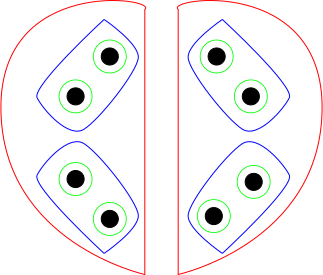
\includegraphics[width=\textwidth]{figs/mongesubgraph.pdf}
    \caption{A decomposition of a DDG into bipartite graphs. The black circles are
    boundary nodes of a piece $P$. The red line splits the vertex set into a bipartite
  graph. The blue and green does the same on a lower level of the recursion. The
decomposition has depth $O(\lg \sqrt{r})$ and each vertex appears in $O(\lg \sqrt{r})$
subgraphs.}
    \label{mongesubgraph}
  \end{subfigure}
  \quad
  \begin{subfigure}[b]{0.45\textwidth}
    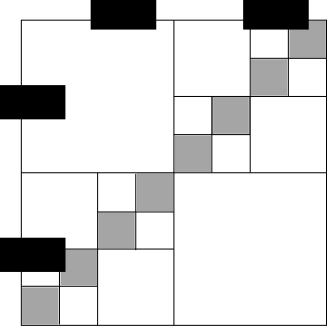
\includegraphics[width=\textwidth]{figs/mongematrix.pdf}
    \caption{A matrix $M$ that is not Monge and a decomposition of $M$ into submatrices
    that all are in Monge. The shaded parts are not in Monge and are to be decomposed
  further. \\ \\ \\ \\}
    \label{mongematrix}
  \end{subfigure}
\end{figure}

\subsection{FR-Djikstra}\label{frdjikstra}
We now describe the fast variant of Djikstra that is the basis for the dynamic distance oracle given in
Section \ref{oracle3}. To build the data structues needed for FR-Djikstra, we use Kaplan
et al. \cite{kaplan2012submatrix} to get $O(n\lg n)$ construction time and space. \\
\\
Fakcharoenphol and Rao \cite{fakcharoenphol2006planar} gave an algorithm for finding
shortest paths in a DDG depending on the number of boundary vertices. For an
$r$-division, the number of boundary nodes is $\beta=O(n/\sqrt{r})$. Note that simply
running Djikstra's algorithm on the DDG would take
$O(\beta^2)$ time. However, they are able to exploit the Monge-like property of the
edges in the DDG to run it in $O(\beta\lg \beta\lg \sqrt{r})$ time. Specifically, the
decomposition of the DDG into bipartite subgraphs gives us a
clique $C$ for each subgraph in the decomposition, for which we store a Monge heap. We
denote these heaps as $M_c$. Besides that, we keep a global heap $H$ to be used in
Djikstra step in which we store references to each Monge heap $M_c$ as well as its
representative vertex $v$ and its label $d_v$. Additionally, for each vertex $v$, we
record if it has been visited before. As mentioned in
Section \ref{mongeheap}, we can have up to $O(\lg \sqrt{r})$ copies of each vertex in the
Monge heaps, though we only do something the first time it is extracted. \\
This suffices to explain the query algorithm in FR-Djikstra. In each iteration of
Djikstra, we extract the minimum element, call it $v$, from the global heap $H$. If it has been visited
before, we do nothing except extracting it. If it has not been visited, we mark it as
visited and set the distance $d(s,v)$ for a source $s$ to be equal to $d_v$ (in $H$). For
each Monge heap that $v$ was part of, $M_{c'}$, we perform \texttt{scanInPiece($v$,
$d_v$)} followed by a call to \texttt{findMin()}. If $v$ was the representative of a Monge
heap, we extract it as well and find a new representative with \texttt{findMin()}. The
global heap is updated accordingly by inserting the new minimum element from $M_{c'}$. \\
\\
Note that every time we call \texttt{findMin()}, we either call \texttt{extractMin()} or
\texttt{scanInPiece()}, which means we can bound the running time in the number of calls to
\texttt{extractMin()} and \texttt{scanInPiece()}. Any vertex $v$ is extracted at most
$O(\lg \sqrt{r})$ as it belongs to at most $O(\lg \sqrt{r})$ Monge heaps. We also only
perform \texttt{scanInPiece()} once for every vertex in each Monge heap. Thus, this
requires $O(\lg^2 \sqrt{r})$ time for each vertex. There is a total of $\beta$ boundary
vertices, so the total time of this is $O(\beta\lg^2 \sqrt{r})$. \\
The number of vertices in the global heap $H$ at any point is $O(\beta)$, so finding the
minimum element takes $O(\lg \beta)$ time. Each vertex is inserted into $H$ at most $O(\lg
\sqrt{r})$ times, so the number of extractions from $H$ is $O(\beta\lg \sqrt{r})$. Thus we
can run Djikstra in $O(\beta\lg \beta\lg \sqrt{r})$ time.

\subsection{Additively weighted Voronoi diagrams}
A point location method used in the oracle described in Section \ref{oracle2} is based on
\textit{additively weighted Voronoi diagrams} which is what allows us to perform faster
queries. \\
When we find a Jordan curve which split the region $R$ into subregions $P$ and $Q$, we
define an additively weighted Voronoi diagram from a vertex $u\in P$ and a hole
$h$ in $Q$. We write $VD(u,h)$ to denote the diagram. The sites of the Voronoi diagram
are the boundary vertices of the hole $h$. A vertex $v$ in the interior of $h$ belongs to
the Voronoi cell given by boundary node $b_i$ (site) if the distance from $u$ to $b_i$
plus the distance from $b_i$ to $v$ is less
than the same distance through all other boundary vertex. We make the simplifying
assumption that all cells are non-empty. This assumption, however, can be overcome
without getting worse asymptotic running time \cite{gawrychowski2017better}.  \\
The representation we are interested in is the one given by the dual $VD^*(u,h)$, where
each face in the primal graph (which we assume is fully triangulated) correspond to a
vertex in $VD^*$ and there is an edge in $VD^*$ whenever two faces share an edge in the
primal graph. We further contract edges in $VD^*$ incident to vertices of degree two.
This ensures that all vertices have degree three (faces that are incident to three
vertices of the primal graph which all belong to different sites in the Voronoi diagram
$VD$. Figure \ref{awvd1} and \ref{awvd2} illustrates this for a hole $h$. \\
\begin{figure}
  \centering
  \begin{subfigure}[b]{0.45\textwidth}
    \includegraphics[width=\textwidth]{figs/awvd1.pdf}
    \caption{Illustration of an additively weighted Voronoi diagram $VD(u,h)$. The hole
    $h$ is shown with boundary vertices in black, interior vertices in grey. Any shortest path
  from $u$ (not shown) to an interior vertex must go through the boundary vertex whose
cell the interior vertex belongs to.}
    \label{awvd1}
  \end{subfigure}
  \quad
  \begin{subfigure}[b]{0.45\textwidth}
    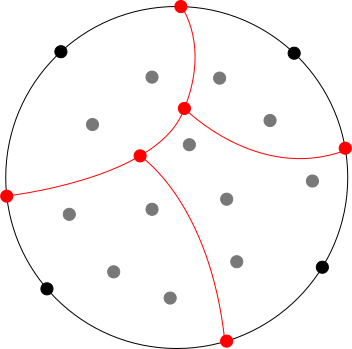
\includegraphics[width=\textwidth]{figs/awvd2.pdf}
    \caption{Illustration the dual Voronoi diagram $VD^*(u,h)$. The vertices of
      $VD^*$ are the intersection of edges of $VD$ with degree three. The diagram $VD^*$
    is given by red vertices and red edges.\\ \\}
    \label{awvd2}
  \end{subfigure}
  \label{awvd}
\end{figure}
As each hole has $r$ vertices and
$\sqrt{r}$ boundary vertices. The number of vertices in $VD^*$ is $O(\sqrt{r})$ as we
only get another vertex of degree three whenever we add another boundary vertex. Since
$VD^*$ is also planar, it has $O(\sqrt{r})$ edges. An important
note is that there exist a compact representation of $VD^*$ using $O(\sqrt{r})$ space.
